	% Darmstadt|Frankfurt|JuanLesPins
	
	\documentclass{beamer}
	\setbeamertemplate{navigation symbols}{}
	
	\usetheme{hpi}
	\usepackage[ngerman]{babel}
	\usepackage[utf8]{inputenc}
	\usepackage{geometry}
	\usepackage[T1]{fontenc}
	\usepackage{graphicx} %Zum Bilder einbinden
	\usepackage{float} %Damit die Figures, also die Bilder, mitten im Text, an geforceter Position erscheinen
	\usepackage{verbatim} %für mehrzeilige Kommentare \begin~\end{comment}
	\usepackage{amstext} % \text{asdf} in Formeln, statt \mbox, weil mbox die Schriftgröße festsetzt	
	\usepackage{amsmath}
	\usepackage{amssymb}
	\usepackage{ucs}
	\usepackage{BeamerColor}
	
	\usepackage{listings}
	\usepackage{color}
	\usepackage{hyperref}
	\usepackage{acronym}
	\definecolor{tplcolor}{HTML}{F6AE15}
	\usecolortheme[named=tplcolor]{structure}
	
	\lstset{
		language=Java, 
		inputencoding=utf8,
		tabsize=2,
		basicstyle=\tiny,
		captionpos=b,language=JAVA,breaklines=true,      % the size of the fonts that are used for the line-numbers,
		stepnumber=5,   
		keywordstyle=\color{brown},
		commentstyle=\color{DarkGreen}, 
		stringstyle=\color{blue},
		showstringspaces=false,
		breaklines=true
		literate=%
		{Ö}{{\"O}}1
		{Ä}{{\"A}}1
		{Ü}{{\"U}}1
		{ß}{{\ss}}1
		{ü}{{\"u}}1
		{ä}{{\"a}}1
		{ö}{{\"o}}1
		{~}{{\textasciitilde}}1	
	}

	\beamersetuncovermixins{\opaqueness<1>{25}}{\opaqueness<2->{15}}
	
	\usecaptiontemplate{
	\tiny
	\structure{\insertcaptionname~\insertcaptionnumber:}
	\insertcaption
	}
	
	\usefootnotetemplate{
	\tiny
	\parindent 1em\noindent
	\hbox to 1.8em{\hfil\insertfootnotemark}\insertfootnotetext
	}
	\begin{document}
			
	\setbeamercovered{invisible}
	
	\title[Kundenvortrag - Analyseprojekt]{Kundenvortrag - Analyseprojekt\\ Eine Mitgliederverwaltung für den Malteser Hilfsdienst}
	\date{5.6.2018}
	\author{Gruppe 3}
	
	 \begin{frame}[title=Hauptgebaeude_Nacht.jpg]
	 \maketitle
	 \date{22. Mai 2018}
 	\end{frame}
	 
	\begin{frame}
		\frametitle{Gliederung}
		\tableofcontents
		%Folien mit einem * im Titel sollen beim Vortrag übersprungen werden.
	\end{frame}
		
\section{Problembereich}
\subsection{Getroffene Annahmen}		
\begin{frame}
\frametitle{Getroffene Annahmen}
Es sind folgende Annahmen über den Problembereich getroffen worden:
\begin{itemize}
\item Stammdaten können geändert werden, allerdings sind manche dieser Daten (z.B. E-Mail-Adresse) bei einer Änderung zu verifizieren. Andere wiederum können ohne Verifizierung direkt geändert werden.
\item Einsatzleiterausbildungen sind Qualifikationen, auch wenn sie im gegebenen Beispiel als eigene Spalte aufgeführt werden.
\item Fähigkeiten eines Helfers, die nicht urkundlich nachgewiesen werden müssen, werden nicht in der Personalverwaltung aufgeführt
\end{itemize}
\end{frame}

\subsection{Modell des Problembereichs}		
\begin{frame}
\frametitle{Modell des Problembereichs - IST}
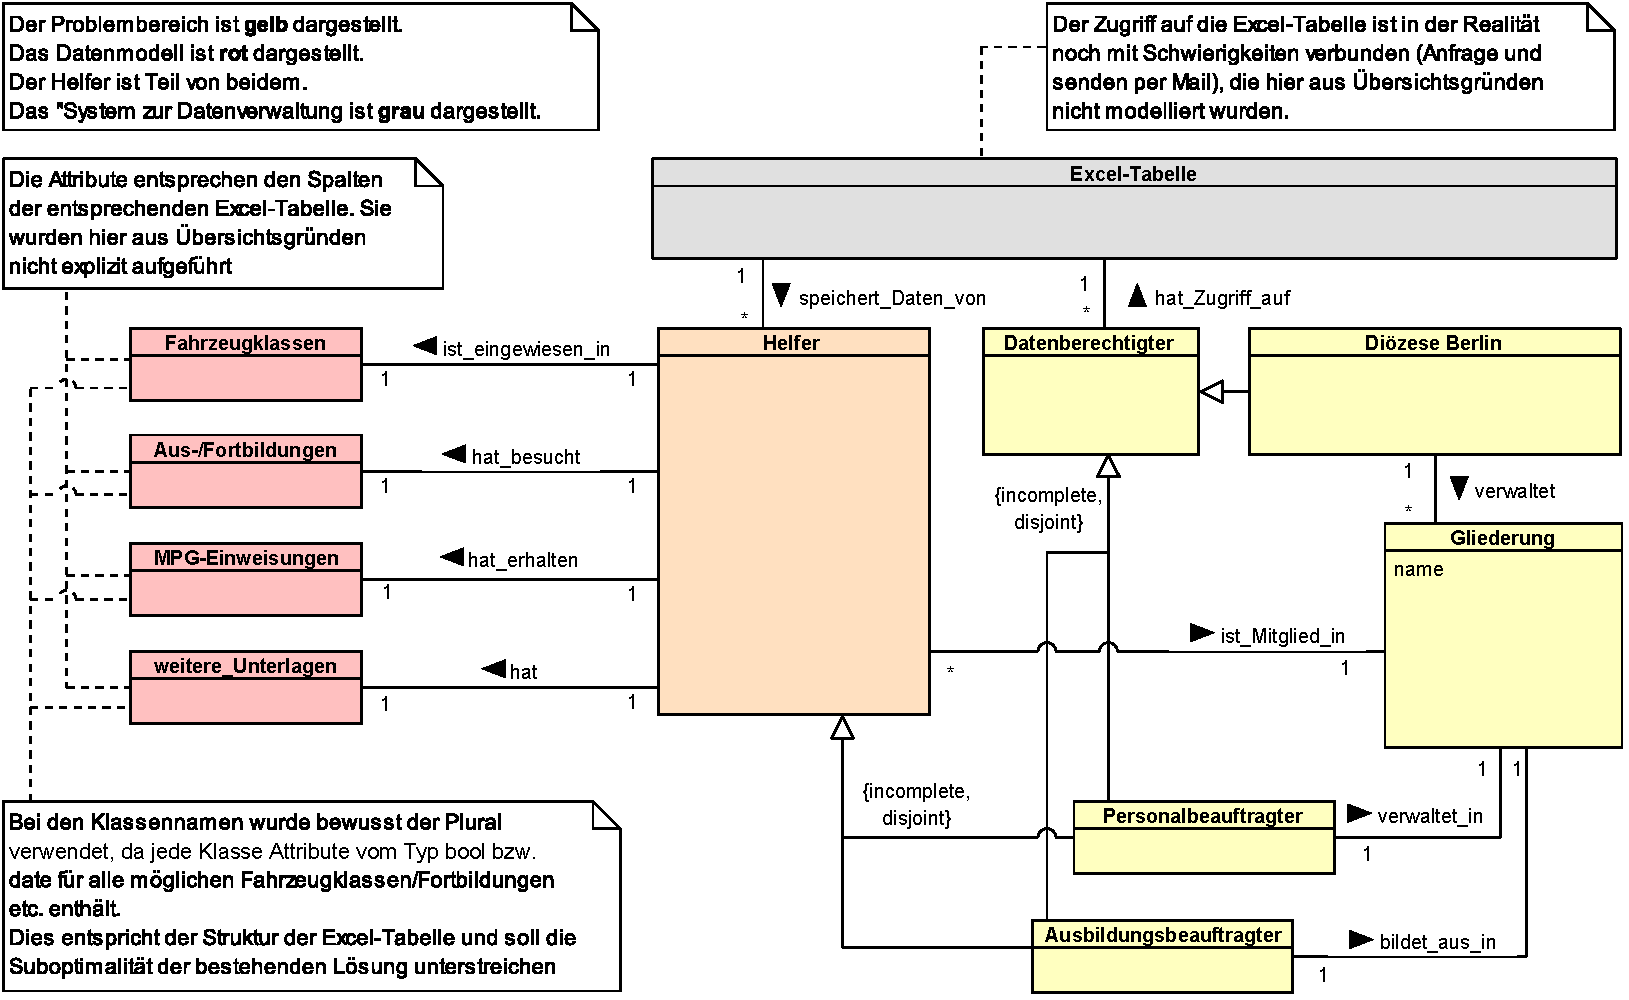
\includegraphics[height=0.75 \textheight]{PDF/Klassendiagramm_ist.pdf}
\end{frame}
\begin{frame}
\frametitle{Modell des Problembereichs - SOLL}
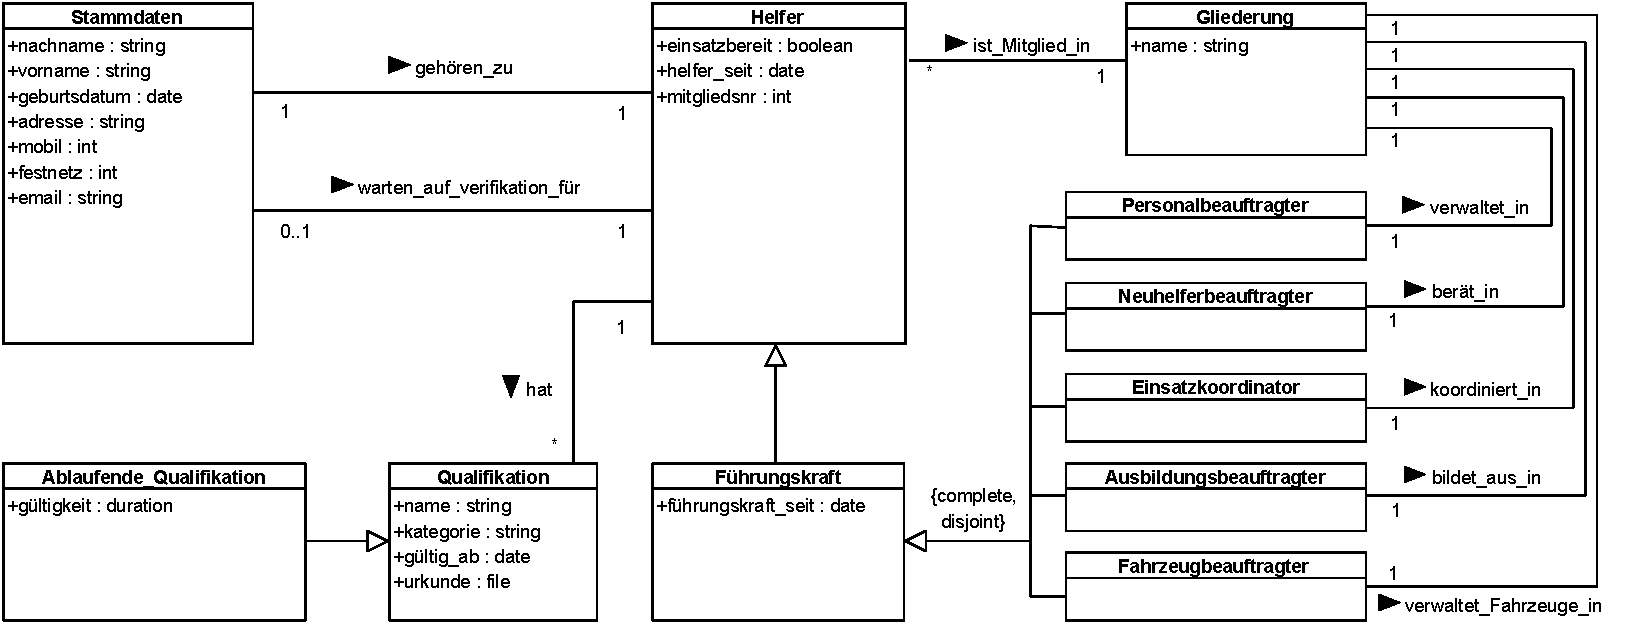
\includegraphics[width=\textwidth]{PDF/Klassendiagramm_soll.pdf}
\end{frame}

\subsection{Geschäftsprozesse}		
\begin{frame}
\frametitle{Den Maltesern beitreten}
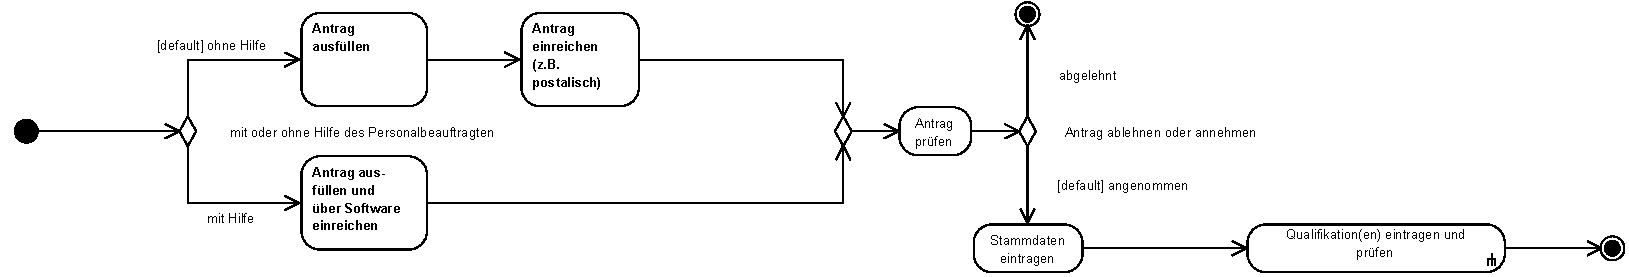
\includegraphics[width=\textwidth]{PDF/BusinessP/Mitglied_werden.pdf}
\end{frame}

\begin{frame}
\frametitle{Personenbezogene Daten ändern}
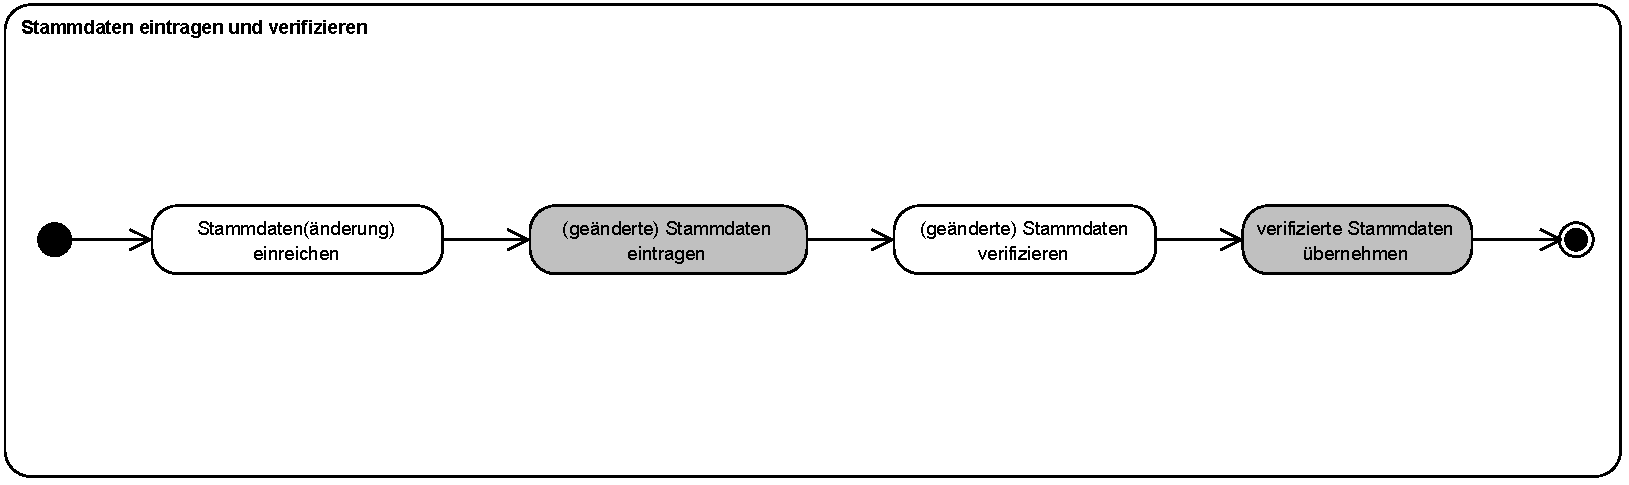
\includegraphics[width=\textwidth]{PDF/BusinessP/Daten_aendern.pdf}
\end{frame}

\begin{frame}
\frametitle{Qualifikation eintragen}
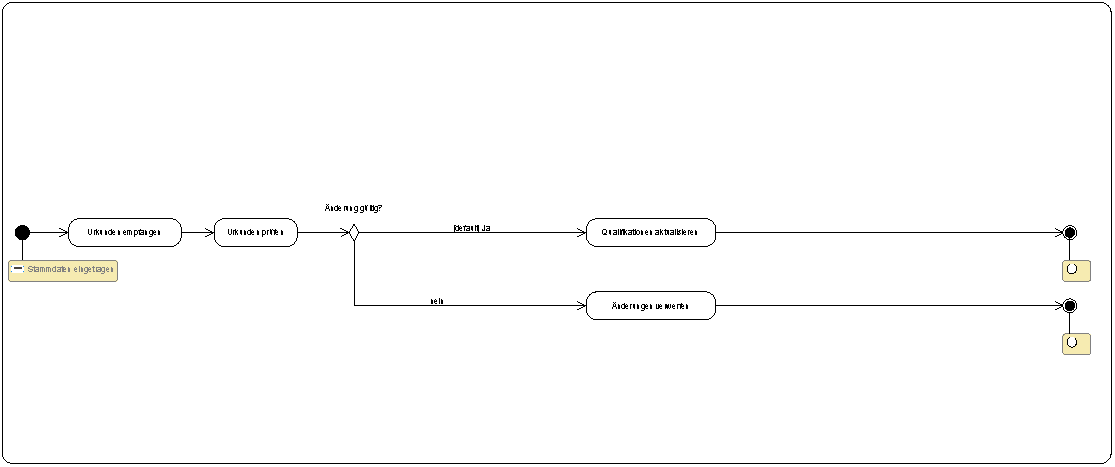
\includegraphics[width=\textwidth]{PDF/BusinessP/Qualifikation_eintragen.pdf}
\end{frame}


\begin{frame}
\frametitle{Ablaufende Qualifikation erneuern}
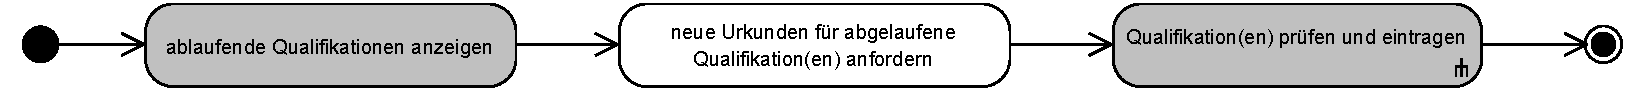
\includegraphics[width=\textwidth]{PDF/BusinessP/Qualifikation_erneuern.pdf}
\end{frame}

\begin{frame}
\frametitle{Aus den Maltesern austreten}
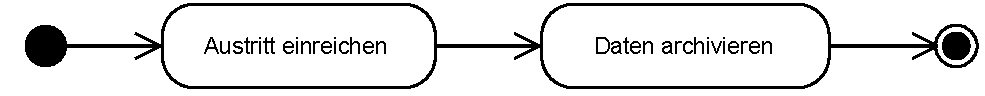
\includegraphics[width=\textwidth]{PDF/BusinessP/Austreten.pdf}
\end{frame}


\section{Produktfunktion}		
\begin{frame}
\frametitle{Produktfunktion}
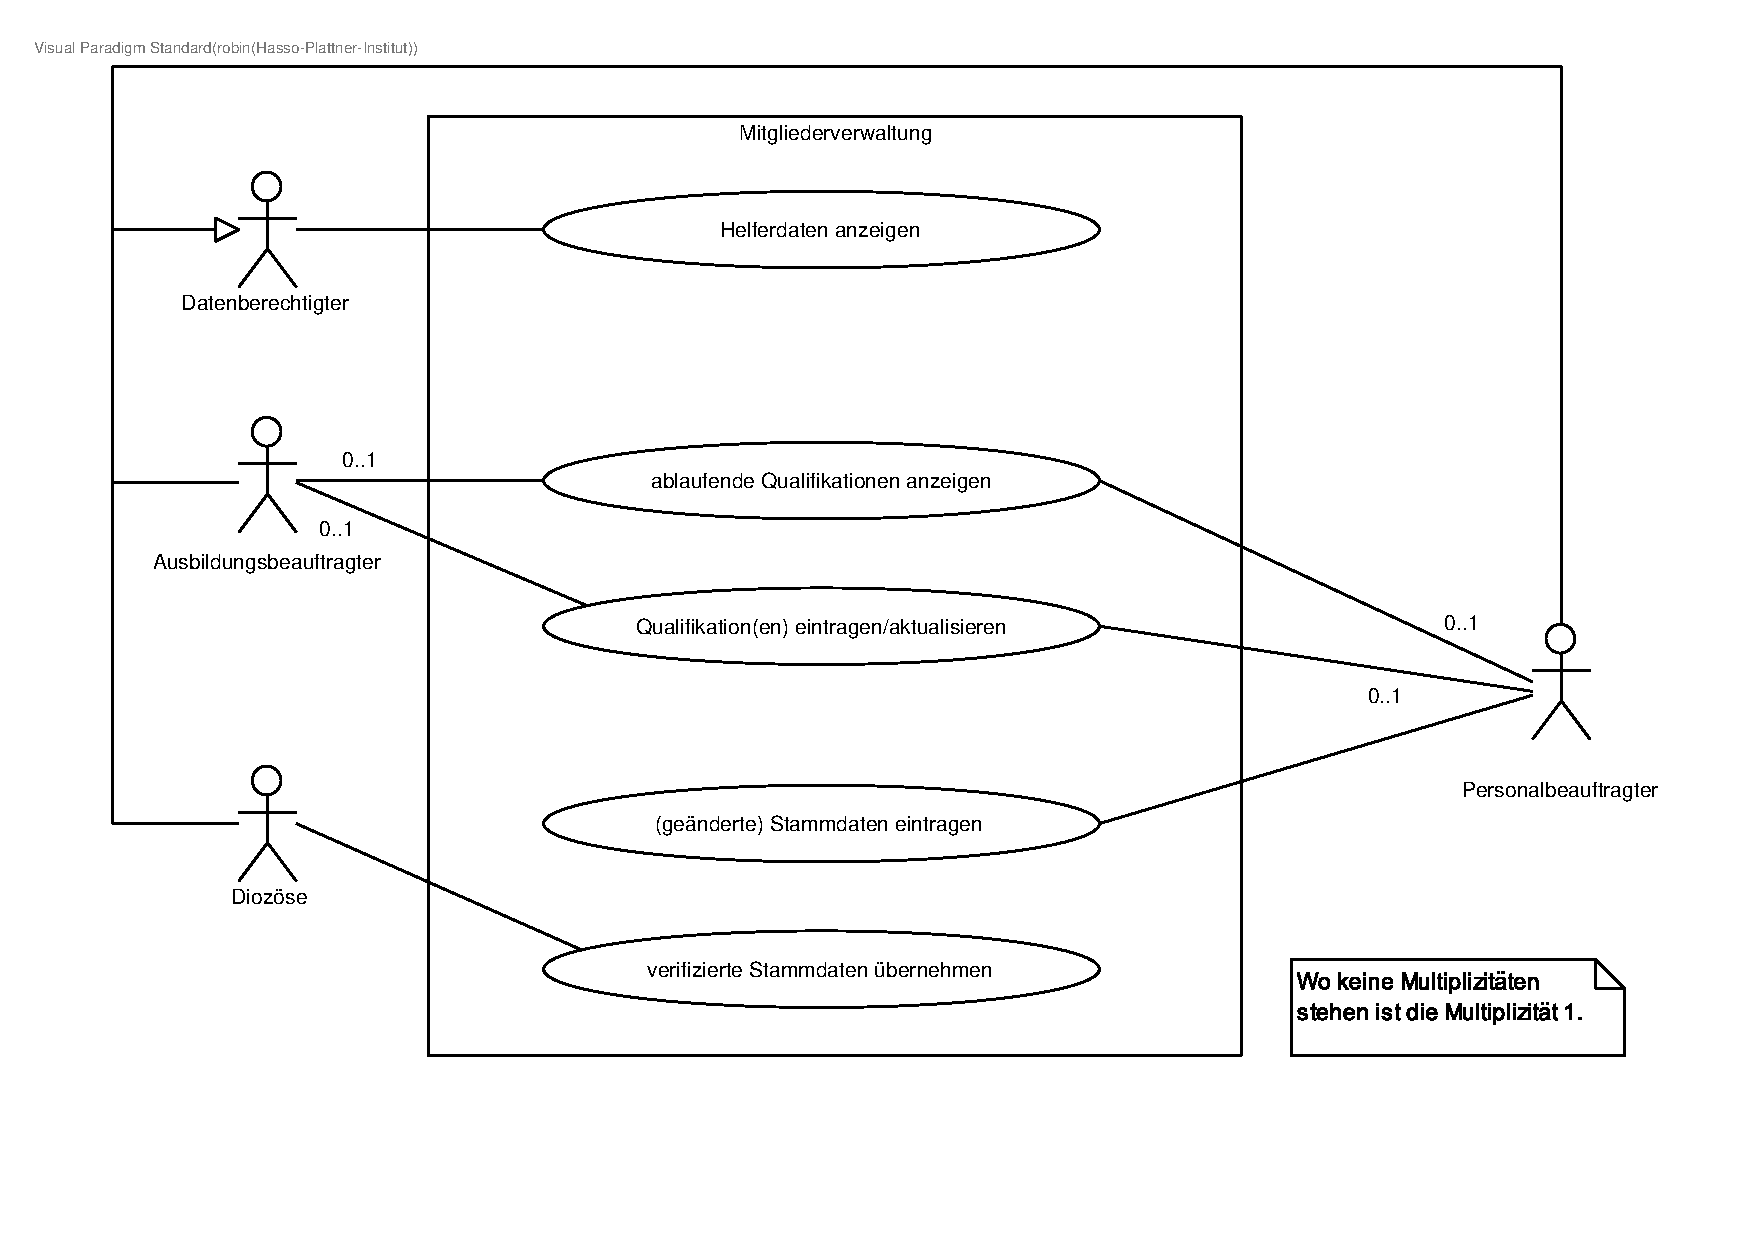
\includegraphics[height=0.75 \textheight]{PDF/Use_Case.pdf}
\end{frame}
	
\begin{frame}[title=Hauptgebaeude_Nacht.jpg]
\maketitle
\date{22. Mai 2018}
\end{frame}
\end{document}

